%%%%%%%%%%%%%%%%%%%%%%%%%%%%%%%%%%%%%%%%%
% University/School Laboratory Report
% LaTeX Template
% Version 3.1 (25/3/14)
%
% This template has been downloaded from:
% http://www.LaTeXTemplates.com
%
% Original author:
% Linux and Unix Users Group at Virginia Tech Wiki 
% (https://vtluug.org/wiki/Example_LaTeX_chem_lab_report)
%
% License:
% CC BY-NC-SA 3.0 (http://creativecommons.org/licenses/by-nc-sa/3.0/)
%
%%%%%%%%%%%%%%%%%%%%%%%%%%%%%%%%%%%%%%%%%

%----------------------------------------------------------------------------------------
%	PACKAGES AND DOCUMENT CONFIGURATIONS
%----------------------------------------------------------------------------------------

\documentclass{article}

\usepackage[version=3]{mhchem} % Package for chemical equation typesetting
\usepackage{siunitx} % Provides the \SI{}{} and \si{} command for typesetting SI units
\usepackage{graphicx} % Required for the inclusion of images
\usepackage{natbib} % Required to change bibliography style to APA
\usepackage{amsmath} % Required for some math elements 
\usepackage{enumerate} % Required for the enumerate function
\usepackage[siunitx]{circuitikz} % Required for the drawing of circuit diagrams
\usepackage{caption}
\usepackage{graphicx}
\usepackage{subcaption}
\usepackage{xfrac}
\usepackage{float}
\usepackage{enumitem}

\setlength\parindent{0pt} % Removes all indentation from paragraphs

\renewcommand{\labelenumi}{\alph{enumi}.} % Make numbering in the enumerate environment by letter rather than number (e.g. section 6)

%\usepackage{times} % Uncomment to use the Times New Roman font

\graphicspath{{./fig/}}

%----------------------------------------------------------------------------------------
%	DOCUMENT INFORMATION
%----------------------------------------------------------------------------------------

\title{Analogue Electronics \\ Experiment 2 - MOSFET Characteristics \\ ENG221} % Title

\author{Shane \textsc{Reynolds}} % Author name

\date{\today} % Date for the report

\begin{document}

\maketitle % Insert the title, author and date

\begin{center}
\begin{tabular}{l r}
Date Performed: & April 8, 2015 \\ % Date the experiment was performed
Instructor: & Dr Sina Vafi % Instructor/supervisor
\end{tabular}
\end{center}

% If you wish to include an abstract, uncomment the lines below
% \begin{abstract}
% Abstract text
% \end{abstract}

%----------------------------------------------------------------------------------------
%	SECTION 1
%----------------------------------------------------------------------------------------

\section{Objective}

To determine the internal parameters of a MOSFET.

\subsection{Background}
\label{definitions}
\begin{description}
\item[Output Resistance in Saturation]
In saturation, the idealised model of the MOSFET tells us that $i_D$ is independent of $v_{DS}$. This implies that some change $\Delta v_{DS}$ means that there is no change in $i_D$, however, this is an idealisation. In reality the device will experience something called channel length modulation. This shrinkage of the length of the channel means that the MOSFET is now modelled by: 

\begin{align}
i_D = \frac{1}{2}k'_{n}\bigg(\frac{W}{L}\bigg)(v_{GS} - V_t)^2(1 + \lambda v_{DS})
\end{align}

where

\begin{description}[labelindent=1cm]
\item $i_D = \text{current through the device}$
\item $\frac{W}{L} = \text{ratio of the device width to the device length}$
\item $k'_n = \text{transconductance parameter}$
\item $v_{GS} = \text{voltage from the gate to the source}$
\item $V_t = \text{threshold voltage}$
\item $\lambda = \text{channel length modulation parameter}$
\item $v_{DS} = \text{the voltage from the drain to the source}$ \\
\end{description}

In equation (1) we see that $i_D$ is linearly dependent on $v_DS$. Extrapolating the model in saturation yields the following formula:

\begin{align}
V_A = \frac{1}{\lambda}
\end{align}

If $i_D$ is now dependent on $v_{DS}$, then for a given $v_{GS}$, a change $\Delta v_{DS}$ yields a change $\delta i_D$ in the drain current $i_D$. Hence we define the output resistance as $r_o$ and express it as:

\begin{align}
r_o = \bigg[ \frac{\partial i_D}{\partial v_{DS}}\bigg]^{-1}_{v_{GS} \text{ constant}}
\end{align}

\end{description} 
 
%----------------------------------------------------------------------------------------
%	SECTION 2
%----------------------------------------------------------------------------------------

\section{Experimental Data}

% Figure 1 with experimental data for Output Characteristic
\begin{figure}[H]
\begin{minipage}{.6\textwidth}
\ctikzset {bipoles/length=.8cm}
\begin{circuitikz}[scale=0.4]
		
		\draw
		node[nmos] (mos) {} (mos.drain)
		to [short, -*] (0,3)
		to [short] (1,3)
		to [generic, l^=$DCM$] (3,3)
		to [short] (4,3)
		to [short] (4,2)
		to [R, l=$R_D$] (4,0)
		;
		
		\draw
		(4,-2) node[ground] {}
		to [battery1, l_=$VDD$] (4,0)
		;
		
		\draw
		(0,-2) node[ground] {}
		to (mos.source)
		;
		
		\draw
		(-4,-5) node[ground] {}
		to [battery1, l=$VGG$] (-4,-3)
		to [R, l=$R_G$] (-4,-1)
		to [short] (-4,0)
		to (mos.gate)
		;
		
\end{circuitikz}
\captionof{figure}{n-type MOSFET circuit}
\label{fig:figure2}
\end{minipage}
\begin{minipage}{.6\textwidth}
\begin{tabular}{ | r | r | r | r | r | }
    \hline
    \multicolumn{1}{|c}{\bfseries $VDD$}
    & \multicolumn{1}{|c}{\bfseries $VGG$}
    & \multicolumn{1}{|c}{\bfseries $V_{R_D}$}
    & \multicolumn{1}{|c}{\bfseries $\sfrac{V_{R_D}}{R_D}$}
    & \multicolumn{1}{|c|}{\bfseries $V_D$} \\ \hline
    %$VDD$ & $VGG$ & $V_{R_D}$ & $\sfrac{V_{R_D}}{R_D}$ & $V_D$ \\ \hline
    10.00 \si{\volt} & 1.3 \si{\volt} & 0 \si{\volt} & 0 \si{\milli\ampere} & 10.00 \si{\volt} \\ \hline
    10.00 \si{\volt} & 2.00 \si{\volt} & 0.38 \si{\volt} & 0.38 \si{\milli\ampere} & 9.62 \si{\volt} \\ \hline
    8.00 \si{\volt} & 2.00 \si{\volt} & 0.38 \si{\volt} & 0.38 \si{\milli\ampere} & 9.62 \si{\volt} \\ \hline
    6.00 \si{\volt} & 2.00 \si{\volt} & 0.38 \si{\volt} & 0.38 \si{\milli\ampere} & 9.62 \si{\volt} \\ \hline
    4.00 \si{\volt} & 2.00 \si{\volt} & 0.38 \si{\volt} & 0.38 \si{\milli\ampere} & 9.62 \si{\volt} \\ \hline
    2.00 \si{\volt} & 2.00 \si{\volt} & 0.38 \si{\volt} & 0.38 \si{\milli\ampere} & 9.62 \si{\volt} \\ \hline
    10.00 \si{\volt} & 3.00 \si{\volt} & 1.58 \si{\volt} & 1.58 \si{\milli\ampere} & 8.42 \si{\volt} \\ \hline
    8.00 \si{\volt} & 3.00 \si{\volt} & 1.58 \si{\volt} & 1.58 \si{\milli\ampere} & 8.42 \si{\volt} \\ \hline
    6.00 \si{\volt} & 3.00 \si{\volt} & 1.58 \si{\volt} & 1.58 \si{\milli\ampere} & 8.42 \si{\volt} \\ \hline
    4.00 \si{\volt} & 3.00 \si{\volt} & 1.58 \si{\volt} & 1.58 \si{\milli\ampere} & 8.42 \si{\volt} \\ \hline
    2.00 \si{\volt} & 3.00 \si{\volt} & 1.36 \si{\volt} & 1.36 \si{\milli\ampere} & 8.64 \si{\volt} \\ \hline
    10.00 \si{\volt} & 4.00 \si{\volt} & 3.48 \si{\volt} & 3.48 \si{\milli\ampere} & 6.52 \si{\volt} \\ \hline
    8.00 \si{\volt} & 4.00 \si{\volt} & 3.48 \si{\volt} & 3.48 \si{\milli\ampere} & 6.52 \si{\volt} \\ \hline
    6.00 \si{\volt} & 4.00 \si{\volt} & 3.48 \si{\volt} & 3.48 \si{\milli\ampere} & 6.52 \si{\volt} \\ \hline
    4.00 \si{\volt} & 4.00 \si{\volt} & 3.48 \si{\volt} & 3.48 \si{\milli\ampere} & 6.52 \si{\volt} \\ \hline
    2.00 \si{\volt} & 4.00 \si{\volt} & 2.51 \si{\volt} & 2.51 \si{\milli\ampere} & 7.49 \si{\volt} \\ \hline
    10.00 \si{\volt} & 5.00 \si{\volt} & 5.56 \si{\volt} & 5.56 \si{\milli\ampere} & 4.40 \si{\volt} \\ \hline
    8.00 \si{\volt} & 5.00 \si{\volt} & 5.56 \si{\volt} & 5.56 \si{\milli\ampere} & 4.40 \si{\volt} \\ \hline
    6.00 \si{\volt} & 5.00 \si{\volt} & 5.56 \si{\volt} & 5.56 \si{\milli\ampere} & 4.40 \si{\volt} \\ \hline
    4.00 \si{\volt} & 5.00 \si{\volt} & 5.20 \si{\volt} & 5.20 \si{\milli\ampere} & 4.80 \si{\volt} \\ \hline
    2.00 \si{\volt} & 5.00 \si{\volt} & 3.33 \si{\volt} & 3.33 \si{\milli\ampere} & 6.67 \si{\volt} \\ \hline
\end{tabular}
\captionof{table}{Output characteristic}
\end{minipage}
\end{figure}

% Figure 2 with experimental data for output resistance
\begin{figure}[H]
\centering
\begin{minipage}{.7\textwidth}
\begin{tabular}{ | r | r | r | r | r |}
    \hline
    $VDD$ & $VGG$ & $V_{R_D}$ & $\sfrac{V_{R_D}}{R_D}$ & $V_D$\\ \hline
    10.50 \si{\volt} & 5.00 \si{\volt} & 5.5 \si{\volt} & 5.5 \si{\milli\ampere} & 5 \si{\volt}\\ \hline
    15.6 \si{\volt} & 5 \si{\volt} & 5.56 \si{\volt} & 5.56 \si{\milli \ampere} & 10 \si{\volt}\\ \hline
\end{tabular}
\captionof{table}{Output resistance}
\end{minipage}
\end{figure}

% Figure 3 with experimental data for control characteristic
\begin{figure}[H]
\begin{minipage}{.5\textwidth}
\begin{tabular}{ | r | r | }
    \hline
    $v_{GS}$ & $i_D$ \\ \hline
     1.3 \si{\volt} & 10 \si{\milli \ampere}  \\ \hline
     1.4 \si{\volt} & 40 \si{\milli \ampere}  \\ \hline
     1.5 \si{\volt} & 70 \si{\milli \ampere}  \\ \hline
     1.6 \si{\volt} & 110 \si{\milli \ampere}  \\ \hline
     1.7 \si{\volt} & 140 \si{\milli \ampere}  \\ \hline
     2.0 \si{\volt} & 360 \si{\milli \ampere}  \\ \hline
     3.0 \si{\volt} & 1560 \si{\milli \ampere}  \\ \hline
     4.0 \si{\volt} & 3240 \si{\milli \ampere}  \\ \hline
     5.0 \si{\volt} & 3710 \si{\milli \ampere}  \\ \hline
\end{tabular}
\captionof{table}{Control $V_{DD} = 5 \si{\volt}$}
\end{minipage}
\begin{minipage}{.5\textwidth}
\begin{tabular}{ | r | r | }
    \hline
    $v_{GS}$ & $i_D$ \\ \hline
      1.3 \si{\volt} & 20 \si{\milli \ampere}  \\ \hline
      1.4 \si{\volt} & 30 \si{\milli \ampere}  \\ \hline
      1.5 \si{\volt} & 50 \si{\milli \ampere}  \\ \hline
      1.6 \si{\volt} & 80 \si{\milli \ampere}  \\ \hline
      1.7 \si{\volt} & 130 \si{\milli \ampere}  \\ \hline
      2.0 \si{\volt} & 320 \si{\milli \ampere}  \\ \hline
      3.0 \si{\volt} & 670 \si{\milli \ampere}  \\ \hline
      4.0 \si{\volt} & 740 \si{\milli \ampere}  \\ \hline
      5.0 \si{\volt} & 780 \si{\milli \ampere}  \\ \hline
\end{tabular}
\captionof{table}{Control $V_{DD} = 1 \si{\volt}$}
\end{minipage}
\end{figure}

\begin{figure}[H]
\begin{minipage}{.5\textwidth}
\begin{tabular}{ | r | r | }
    \hline
    $v_{GS}$ & $i_D$ \\ \hline
      1.3 \si{\volt} & 10 \si{\milli \ampere}  \\ \hline
      1.4 \si{\volt} & 30 \si{\milli \ampere}  \\ \hline
      1.5 \si{\volt} & 70 \si{\milli \ampere}  \\ \hline
      1.6 \si{\volt} & 100 \si{\milli \ampere}  \\ \hline
      1.7 \si{\volt} & 150 \si{\milli \ampere}  \\ \hline
      2.0 \si{\volt} & 390 \si{\milli \ampere}  \\ \hline
      3.0 \si{\volt} & 1610 \si{\milli \ampere}  \\ \hline
      4.0 \si{\volt} & 3350 \si{\milli \ampere}  \\ \hline
      5.0 \si{\volt} & 5460 \si{\milli \ampere}  \\ \hline
\end{tabular}
\captionof{table}{Control $V_{DD} = 10 \si{\volt}$}
\end{minipage}
\end{figure}

\newpage

%----------------------------------------------------------------------------------------
%	SECTION 3
%----------------------------------------------------------------------------------------

\section{Calculations}

\subsection{Output Resistance}
In the second task we are asked to find the resistance to which the characteristic slope corresponds. According to equation (3) we see that the output resistance is the inverse of the slope of the $i_D$-$v_DS$ line when operating in the saturation region. Hence from equation (3), for a given $v_{GS}$ we can say that:
\begin{align*}
r_o = \frac{\Delta v_{DS}}{\Delta i_D}
\end{align*}

Using the experimental data in table 2 we see that:
\begin{align*}
r_o &= \frac{10 - 5}{5.56\mbox{\sc{e}-}3 - 5.5\mbox{\sc{e}-}3}\\
&= 83.88 \si{\kilo \ohm}
\end{align*}

Now the drain to source was shunted with a resistor of magnitude 83.33 \si{\kilo \ohm}. The previous change in current was:
\begin{align*}
\Delta i_{D_1} = 5.56 \si{\milli \ampere} - 5.5 \si{\milli \ampere} = 0.06 \si{\milli \ampere}
\end{align*}

The change in current with the shunt added was:
\begin{align*}
\Delta i_{D_2} = 5.62 \si{\milli \ampere} - 5.56 \si{\milli \ampere} = 0.06 \si{\milli \ampere}
\end{align*}

Now, if $V_G = V_{DS} = 5 \si{\volt}$, then the shut resistor should be the same value as above: 83.33 \si{\kilo \ohm}. This is because $V_G$ is unchanged. The theory outlined in the background tells us that provided the device is operating in saturation, for some given $V_G$, then $i_D$ and $v_{DS}$ are linearly related. This means that the slope is constant, which in turn implies that the output resistance is constant for a given $V_{GS}$.\\

Now to determine $V_A$ and $\lambda$ we need to determine the equation of the linear relation between $i_D$ and $v_{DS}$. The slope is simply the inverse of the resistance, hence:
\begin{align*}
i_d = \frac{1}{83.33\mbox{\sc{e}}3}v_{DS} + \text{constant}
\end{align*}

To find the constant, we can use the tuple $(i_D, v_{DS}) = (5.56\si{\milli \ampere}, 10 \si{\volt})$:

\begin{align*}
5.56\si{\milli \ampere} &= \frac{1}{83.33\mbox{\sc{e}}3} \times 10 \si{\volt} + \text{constant}\\
\text{constant} &= 46.33
\end{align*}

Hence the equation is:
\begin{align*}
i_d = \frac{1}{83.33\mbox{\sc{e}}3}v_{DS} + 46.33
\end{align*}

Setting $i_D = 0$ and solving for $v_{DS}$ will give us the value for $V_A$. Hence:
\begin{align*}
V_A = 3860678\si{\volt}
\end{align*}

Finally, using equation (2) we can solve for the channel length modulation parameter, $\lambda$:
\begin{align*}
\lambda = \frac{1}{V_A} = \frac{1}{3860678} = 2.59\mbox{\sc{e}-}7
\end{align*}

\subsection{Control Characteristics}
To find the device parameters $k_n$ and $V_t$, we consider two of the experimental data points in table 3. The two points, give us two distinct instances of equation (1), where the modulation parameter, $\lambda$, is assumed to be zero. Now, the equations are:
\begin{align}
i_{D_1} = \frac{1}{2}k'_n(V_{GS_1} - V_t)^2\\
i_{D_2} = \frac{1}{2}k'_n(V_{GS_2} - V_t)^2
\end{align}

If we divide equation (4) by equation (5) we get:
\begin{align*}
\frac{i_{D_1}}{i_{D_2}} = \frac{\frac{1}{2}k'_n(V_{GS_1} - V_t)^2}{\frac{1}{2}k'_n(V_{GS_2} - V_t)^2}\\
\end{align*}

Cancelling the $\frac{1}{2}k'_n$ from the numerator and denominator, we get:
\begin{align*}
\frac{i_{D_1}}{i_{D_2}} = \bigg(\frac{V_{GS_1} - V_t}{V_{GS_2} - V_t}\bigg)^2
\end{align*}

With some algebraic manipulation we arrive at the following relationship:
\begin{align*}
V_T = \frac{\sqrt{\frac{i_{D_1}}{i_{D_2}}}V_{GS_2} - V_{GS_1}}{(\sqrt{\frac{i_{D_1}}{i_{D_2}}} - 1)}
\end{align*}

Using the two points $(1.3\si{\volt}, 20\si{\milli \ampere})$, and $((3\si{\volt}, 670\si{\milli \ampere}))$, we get:
\begin{align*}
V_T = 0.944V
\end{align*}

Hence, we can now solve for $k_n$:
\begin{align*}
k_n = \frac{2i_D}{(V_{GS} - V_T)^2} = 315.6\frac{\si{\milli \ampere}}{\si{\volt}^2}
\end{align*}

%----------------------------------------------------------------------------------------
%	SECTION 4
%----------------------------------------------------------------------------------------

\section{Results and Conclusions}

\subsection{Output Resistance}
The value which was calculated from the experimental data for the output resistance was 83.33\si{\kilo \ohm}. The value for $V_A$ is 3860678\si{\volt} which is very large and consequently the value found for $\lambda$, 2.59\mbox{\sc{e}-}7, is very small. The value for $V_A$ is most likely incorrect as comparable circuits operate with $V_A$ which is many orders of magnitude smaller that the one calculated. The values of both $V_A$ are artefacts of the value chosen for shunt resistor.\\

The shunt resistor values was matched to the output resistance $r_o$, but this is very large when compared to the value of the resistance $R_D$ in the circuit, despite providing the same incremental change in device current $i_D$. The selection of the shunt resistor (and even the value of the output resistance) are most likely erroneous. This is due to misconception and lack of understanding with respect to the fundamental operation of the circuit and how to derive the underlying parameters of the device.

\subsection{Control Characteristics}

The experimental data from table 3, 4 and 5 was plotted in Matlab and can be seen in figures 2, 3 and 4 respectively. The values of $V_t$ that was estimated was 0.944\si{\volt} and the value of $k_n$ that was estimated using $V_t$ was 315.6 $\frac{\si{\milli \ampere}}{\si{\volt}^2}$. The value for $V_t$ is significantly greater than the standard 25 \si{\milli \volt} and hence the calculated value for $V_t$ and $k_n$ is most likely in error.

\begin{figure}[H]
\begin{minipage}{.6\textwidth}
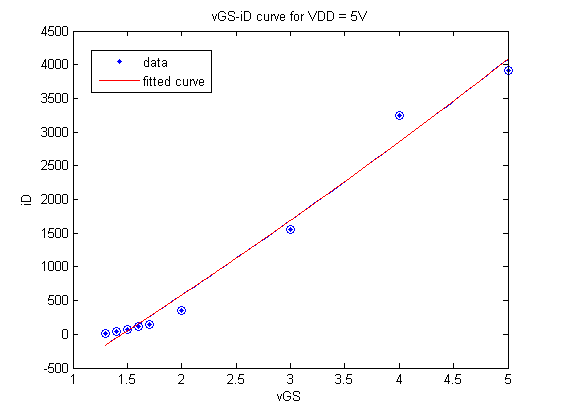
\includegraphics[scale=.4]{fig1}
\captionof{figure}{Plot of $v_{GS} vs. i_D$ for \\$V_{DD} = 5\si{\volt}$}
\end{minipage}
\begin{minipage}{.6\textwidth}
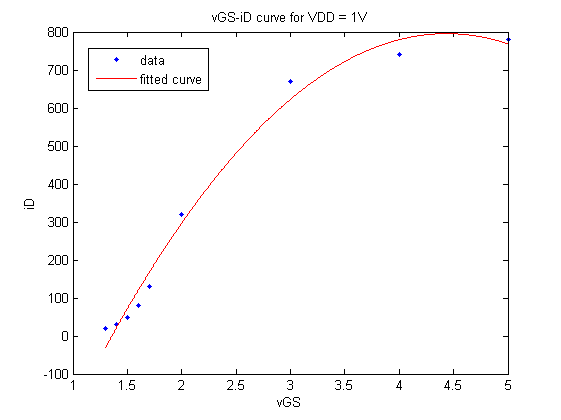
\includegraphics[scale=.4]{fig2}
\captionof{figure}{Plot of $v_{GS} vs. i_D$ for \\$V_{DD} = 1\si{\volt}$}
\end{minipage}
\end{figure}

\begin{figure}[H]
\begin{minipage}{.6\textwidth}
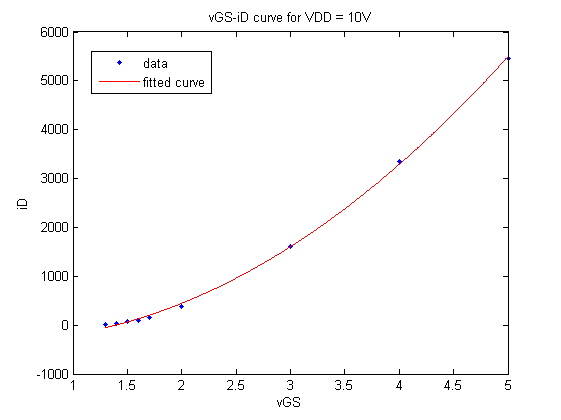
\includegraphics[scale=.4]{fig3}
\captionof{figure}{Plot of $v_{GS} vs. i_D$ for \\$V_{DD} = 10\si{\volt}$}
\end{minipage}
\end{figure}

%----------------------------------------------------------------------------------------
%	BIBLIOGRAPHY
%----------------------------------------------------------------------------------------


%----------------------------------------------------------------------------------------


\end{document}